% Chapter 3

\newglossaryentry{json}{name=JSON, description={JavaScript Object Notation}}

\chapter{Development} % Write in your own chapter title
\label{chap:development}
\lhead{Chapter 3. \emph{Development}} % Write in your own chapter title to set the page header
\begin{flushright}
\textit{``For me, open source is a moral thing.''} \\ Matt Mullenweg
\end{flushright}

In this chapter, we introduce our contribution to the dynamic program analysis. As explained in the introduction the aim is to develop a proof-to-concept system and all the steps to achieve it will be presented in details including the Setup, Data capture model, Data model and its user interface.


\section{Proposed solution}
While working on a growing project, there is always a point where it becomes difficult to keep an eye on all the variables. In order to give the programmer an overview of the variables evolution, this work is aiming to propose a proof-to-concept system which will not only monitor the data evolution, but also give the possibility to compare the gathered data between different runs.

To achieve such a system, the project is going to be separated in three different parts which will constitute the system. First, a data capture model will monitor all the needed variables and their evolution during the execution of the reviewed program. Then a data model will be created and backup procedure will be implemented to store the data in this model. Finally, a web-application will process the extracted data and show them for reviewing the results. Each mentioned part is exposed in the development section.

\section{Environment}
For the project 4 main technologies were chosen in order to develop the required features. 

First the data is captured in \textit{Python} with the help of the integrated Debugger Framework. Python is a widely used high level programming language which has seen these last year an increasing enthusiasm around it, especially for web based applications. Thanks to the dynamic nature of Python, which includes a dynamic type system, the real-time collection of object is a pretty straightforward process and therefore it made plenty sense to use it in our project. More over Python offers good compatibility with other programming language since there are a lot of bindings available. For this project, the newest version 3 of the programming language was chosen because of the better handling of encoding.

Secondly, the extracted data is stored in a \textit{MongoDB} Database. MongoDB is a document-oriented database which enters in the new categorie of No-SQL database systems. MongoDB has the advantage to use \gls{json} like documents with schemas which was a clever choice to store the heterogeneous extracted data.

Finally, the used interface was built with the help of \textit{Python}, \textit{Html/CSS} and \textit{Javascript}. As already said, Python is now an interesting language to develop web applications and was used here, with the help of the Flask framework, for the server side process. HTML/CSS and Javascript were used for the presentation of the results.

Additionally, the chosen IDE was PyCharm academic edition version 2015 and then 2016. PyCharm is a very complete IDE which supports among others Python web frameworks, database support, code inspection. In order to optimize the development management, the GitHub online tool was chosen as version control repository. The deployment during the development of the solution was tested on virtual machine server under Ubuntu Server 14.04. The server is provided by the Department of Informatics at the University of Fribourg and is accessible internally at \url{http://diufpc115.unifr.ch/}. This server will also be used for the experiments in the chapter 5. 
\pagebreak

In order to deploy regularly the newest version of the ongoing work an automation server named Jenkins was configured. Jenkins was charged to fetch every day the latest prototype on the GitHub repository, create a package of it and install it on the server. If during this process a bug occurred, an e-mail to the interested persons was sent.
\begin{figure}[h!]
  \centering
    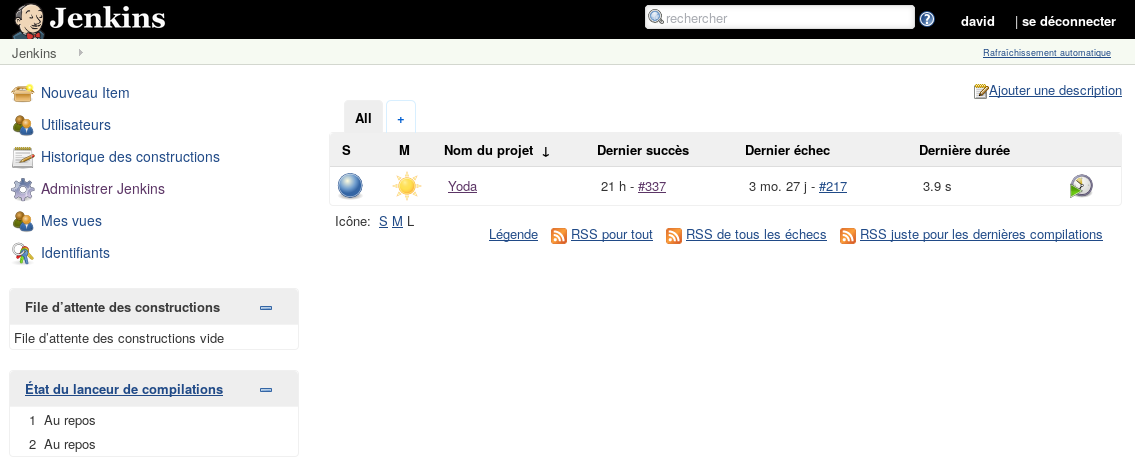
\includegraphics[width=\textwidth]{figures/jenkins.png}
    \caption{The Jenkins home page}
    \label{fig:jenkins}
\end{figure}

In the next section, each module of the proposed system will be exposed in details regarding their functionality and their implementations.

\section{Data Capture Model}
This section is presenting the development phase of the data capture model. The data capture model, or \textit{analyser} as it was called during the development, is the core of the system and is based on the Python Debugger Framework (BDB). BDB handles basic debugger functions, like setting breakpoints or managing execution. Thanks to the object-oriented programming, the classes and the function inheritance, it is a straightforward job to rewrite the different functionality as needed for this project. 

The development began with study of a script provided by Roman Prokofyev which is implementing some basic data capture functionality derived from the Python debugger framework. The understanding of the developed concepts was the first step to the creation of the data capture model. The analyser consists in 240 lines of code and some of the most important functions are explained here.

\subsection{Setting up the trace}
In order to use the analyzer, some code has to be added at the beginning of the aimed file. The code is necessary to import the module and to set the start of the tracing phase. 
\begin{python}
import yoda.analyser
yoda.analyser.db.set_trace()
\end{python}

The \pythoninline{set_trace()} function is inherited by the BDB and is needed to start debugging with a Bdb instance from caller’s frame.
It is also absolutely necessary to stop the trace at the end of the aimed code with the \pythoninline{yoda.analyser.db.set_quit()
} function which set the quitting attribute to \texttt{True}. This raises BdbQuit in the next call to one of the \pythoninline{dispatch_*()} methods. 

For further information about the operating of the Python Debugger Framework, we advise the reader to refer to the official documentation \citep{Foundation2017}.

\subsection{Initialization}

Once the analyser module called, the first step is to setup the \pythoninline{Yoda} class along with some global variables needed during the tracing process. The first variable \pythoninline{json\_results} (line 2) will be explained further but is basically where the extracted data will be stored. Then, the \pythoninline{instrumented\_types} list (line 3) limits the instrumented objects to this list, it is possible to add further objects if needed. The next 6 variables (line 4-9) are needed for gathering and computing line numbers, frames and files name. Finally, the \pythoninline{next_backup} variable (line 10) defines a limit of how many lines can be analyzed before flushing the information in the database.

\begin{python}
class Yoda(bdb.Bdb):
    json_results = None
    instrumented_types = (int, float, str, list, dict)
    prev_lineno = defaultdict(int)
    prev_lineno['<module>'] = 0 
    cur_framename = '<module>'
    file_name = None
    file_id = None 
    total_linenb = 0
    next_backup = 1000
\end{python}

As the needed variables are now set up, the script continues with the initialization of the \pythoninline{Yoda} class. Within the class, the connection of the database is also created if case of production mode (line 4). 

\begin{python}
def __init__(self):
    bdb.Bdb.__init__(self)
    if settings.DEBUG is False:
        mongoengine.connect(settings.MONGODB)
\end{python}

\subsection{Event Catching}

BDB can react to various events during the code execution which are handled by 4 functions : \texttt{user\_call, user\_line, user\_return, user\_exception}. Each function has been rewritten in order to redirect the event to a self-written handling function called \texttt{interaction}. 
\smallskip
\begin{python}
def user_call(self, frame, args):
    self.interaction(frame, 'call', None)
def user_line(self, frame):
    self.interaction(frame, 'line', None)
def user_return(self, frame, value):
    self.interaction(frame, 'return', None)
def user_exception(self, frame, exception):
    self.interaction(frame, 'exception', exception)
\end{python}

Once the \texttt{interaction} function has been called, the first thing to do is to check whenever the \texttt{file\_name} variable is blank or not. If \texttt{file\_name} is \texttt{None} then a new one is taken and applied from the source code file otherwise the script will continue with the handling of the events.
\begin{python}
if self.file_name is None:
    self.file_name = inspect.getfile(frame)
\end{python}

\subsection{Event Handling}
The first handled event type is the \texttt{call} type. This kind of event is normally happening when the frame of the code is changing and thus is really short. Indeed, it just need to capture the frame name (line 2) and catch the line number (line 3). Nothing else special is handled there.
\begin{python}
if event == 'call':
    self.cur_framename = str(frame.f_code.co_name)
    self.prev_lineno[self.cur_framename] = frame.f_lineno
    self.set_step() # continue
\end{python}

Following, the second event type is the the \texttt{line} type which occurs at each line-break. This event is the most important for the data collection and its operating has to be explained in separated steps. First, the interaction function checks the type of the event and then proceed to extract the line number which is a key information for the user interface. Then for each line, the interpreted objects have to be caught. This is handled by a external function called \texttt{\_filter\_locals} and called with the frame locals in option.
\begin{python}
locals = self._filter_locals(frame.f_locals)
\end{python}

The function itself create first an empty dictionary which will store the name and the value of each local (line 2). The locals starting with a double underscore are ignored and only the specified object are fetched (line 4 to 6). The function returns the \texttt{new\_locals} dictionary to the main \texttt{interaction} function (line 9).

\begin{python}
def _filter_locals(self, local_vars):
    new_locals = {}
    for name, value in list(local_vars.items()):
        if name.startswith('__'):
            continue
        if not isinstance(value, self.instrumented_types):
            continue
        new_locals[name] = [copy.deepcopy(value)]
    return new_locals

\end{python}

Then, the locals are stored in a JSON defaultdict object along with the file name, the frame and the line number. At the end, the JSON dictionary is periodically stored in the database in order to flush the data from the memory and enhance the run-time performances. The population of the database is detailed in the next point.

\begin{python}
if self.total_linenb > self.next_backup:
    self._populate_db()
    self.next_backup += self.next_backup
\end{python}

The handling of the \texttt{line} event is now finished and interaction function continues with the two last types. The \texttt{return} event only occurs at the begging of a file for which we just set the main frame name (line 2) and the \texttt{exception} event happens when there is an error in the code which is printed out in the console (line 6).
\begin{python}
if event == 'return':
    self.cur_framename = '<module>'
    self.set_step()  # continue
if event == 'exception':
    name = frame.f_code.co_name or "<unknown>"
    print("exception in", name, exception)
    self.set_continue()  # continue
\end{python}

\subsection{Trace Ending}

Finally, the data capture model is ended by the \pythoninline{set_quit()} BDB function which was remodeled for writing the last traced lines (line 6).
\begin{python}
def set_quit(self):
    self.stopframe = self.botframe
    self.returnframe = None
    self.quitting = True
    sys.settrace(None)

    if self.json_results:
        if settings.DEBUG:
            print(self.json_results)
        else:
            self._populate_db()
\end{python}



\section{Data model}
The data model is an in-between layer used for the Data capture model and the user interface. Both modules parts will be explained in this section along with the presentation of the data model itself.

\subsection{Definition}

\begin{python}
class Line(EmbeddedDocument):
    lineno = IntField()
    data = DictField()
\end{python}
\begin{python}
class Frame(EmbeddedDocument):
    name = StringField()
    lines = ListField(EmbeddedDocumentField(Line))
\end{python}
\begin{python}
class File(Document):
    user = StringField()
    revision = StringField()
    filename = StringField()
    timestamp = DateTimeField()
    content = StringField()
    frames = ListField(EmbeddedDocumentField(Frame))
\end{python}

\subsection{Writing to the database}

\subsection{Reading from the database}
\section{User interface}

The user interface is a web application which helps the programmer to review the result of the data capture model. It is based on the Python web framework Flask intended to be as lightweight as possible.

\begin{python}
from flask import Flask, render_template, redirect, url_for, flash, jsonify
from flask_mongoengine import MongoEngine
from flask_debugtoolbar import DebugToolbarExtension

app = Flask(__name__)
app.config['MONGODB_DB'] = settings.MONGODB
app.config['SECRET_KEY'] = "xxx"
app.debug = True
if __name__ == "__main__":
    app.run()
\end{python}

\subsection{Index page}
\begin{python}
@app.route("/")
def index():
    return render_template('index.html', files=File.objects.exclude("frames", "content").order_by('-timestamp'))
\end{python}

\subsection{Viewing a file}

\subsection{Comparing files}

\section{Concluding remarks}
